\subsection{Dashboard}

La web application oggetto del tirocinio è inerente solamente ai singoli nodi per la loro configurazione e per la consultazione dei dati raccolti. Pertanto, si è pianificato di implementare nel futuro una \emph{dashboard} operativa relativa al server di elaborazione centrale, che raccolga i dati da tutti i nodi e possa permettere all'utente una panoramica generale di tutta la rete PRISMA, per consultare anche gli eventi veri e propri generati dall'elaborazione delle detection.

\subsection{Realtà aumentata}

L'elaborazione dei dati raccolti dalle telecamere della rete, attraverso l'analisi delle immagini e il calcolo delle traiettorie e della magnitudine, genera dei file che riproducono tridimensionalmente l'evento (cfr. figura \ref{fig:bolide-050322}). A fronte di questo, l'INAF ha proposto di creare alcune esperienze in realtà aumentata per gli appassionati o per i più piccoli che riproducano in 3D la caduta della meteora.

\begin{figure}
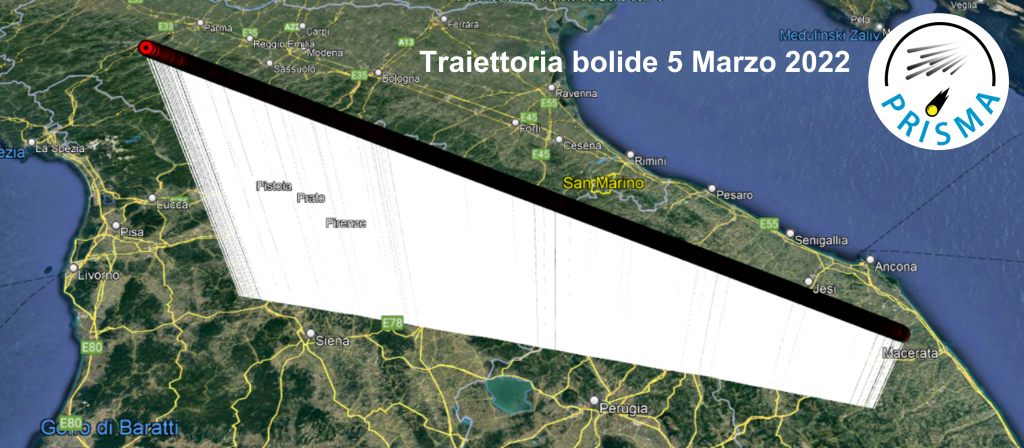
\includegraphics[width=\textwidth]{images/traiettoria-20220305.png}
\caption{Traiettoria del bolide del 5 marzo 2022. \cite{bolide-050322}}
\label{fig:bolide-050322}
\end{figure}

\subsection{Cloud computing}

Attualmente la rete PRISMA si appoggia per l'elaborazione ad un server centrale. Per il futuro si ha intenzione di spostare parte dell'analisi dei dati sui nodi della rete, in modo da non sovraccaricare un unico server e sfruttare la potenza computazionale di ciascuna delle macchine che compongono la rete. In particolar modo, si è pensato di far elaborare i dati dai nodi nelle ore diurne, quando il software FreeTure non è attivo.

\subsection{Integrazione con modelli AI}

Ad oggi, PRISMA basa tutte le sue elaborazioni dai dati raccolti mediante il software open-source FreeTure. È però in corso, sempre in collaborazione con l'azienda N3 Srl, una ricerca sull'implementazione di modelli di intelligenza artificiale più precisi ed efficienti rispetto a FreeTure. 